\chapter{Gestión de Proyectos}

Scrum es un marco de gestión de proyectos para el desarrollo incremental de productos, valiéndose de equipos autoorganizados. A diferencia de la metodología clásica en que la planificación estaba al inicio y el desarrollo en la fase de ejecución, en este marco la planificación se distribuye durante todo el ciclo de vida del proyecto y en la fase de ejecución se hace el desarrollo incremental de productos (por incrementos de producto) en iteraciones cortas (Sprint) donde cada iteración tiene su respectiva planificación (ver figura \ref{fig:ScrumProject}).

\begin{figure}[h]
  \centering
  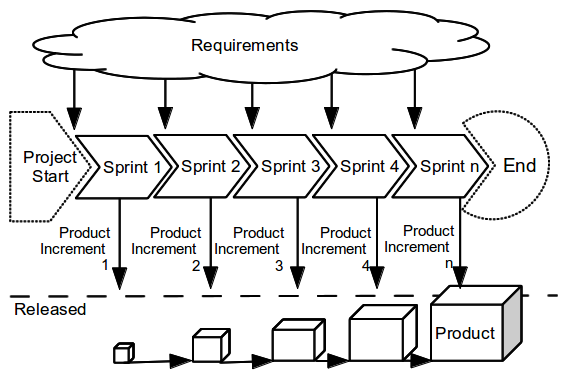
\includegraphics[width=0.90\textwidth]{ScrumProject}
  \caption{Proyecto Scrum}
  \centering
  \label{fig:ScrumProject} %\ref{fig:ScrumProject}
\end{figure}

\subsection{Planificación de entregables}
Con esta metodología tampoco es necesario hacer una entrega final (o "releasing") ya que se pueden hacer entregas paulatinas.

